\section{Numerical simulation}\label{sec:sim}

The model of \cref{sec:model} was implemented in Python with NumPy only
(package \texttt{balancebot}), integrated numerically, verified with a set of
automated tests, and used for a first experiment: the free fall of the robot
with the motor off.

\subsection{State-space form}

The equations of motion are second order in $\q$. Stacking positions and
velocities into the state
\begin{equation}
  \bm{s} = \begin{bmatrix} \q \\ \qd \end{bmatrix}
  = \begin{bmatrix} x & \theta & \dot x & \dot\theta \end{bmatrix}^{\mathsf T}
\end{equation}
turns them into a first-order system $\dot{\bm s} = \bm f(\bm s, \tau)$. The
first two components of $\dot{\bm s}$ are the velocities, already contained in
$\bm s$; the last two are the accelerations, obtained from \cref{eq:manipulator}:
\begin{equation}
  \bm f(\bm s, \tau) = \begin{bmatrix} \qd \\ \qdd \end{bmatrix},
  \qquad \M(\q)\,\qdd = \B\tau - \h(\q,\qd) .
  \label{eq:forward}
\end{equation}
The accelerations are computed by solving this $2\times2$ linear system rather
than by inverting $\M$; the system always has a unique solution because
$\det\M > 0$ (\cref{sec:model}). In the simulation loop the torque is computed
once per step and held constant during the step (zero-order hold), as a digital
controller does.

\subsection{Numerical integration}

\Cref{eq:forward} has no closed-form solution, so the state is advanced in
steps of length $\Delta t$. Two integrators were implemented.

\paragraph{Explicit Euler.} The rate of change at the beginning of the step is
assumed constant over the whole step:
\begin{equation}
  \bm s_{k+1} = \bm s_k + \Delta t\, \bm f(\bm s_k) .
\end{equation}

\paragraph{Fourth-order Runge--Kutta (RK4).} The rate of change is evaluated
four times inside the step, at the start ($\bm k_1$), twice at mid-step
($\bm k_2$, $\bm k_3$) and at the end ($\bm k_4$), and averaged with weights
$1,2,2,1$:
\begin{equation}
\begin{aligned}
  \bm k_1 &= \bm f(\bm s_k), &
  \bm k_2 &= \bm f\big(\bm s_k + \tfrac{\Delta t}{2}\bm k_1\big), \\
  \bm k_3 &= \bm f\big(\bm s_k + \tfrac{\Delta t}{2}\bm k_2\big), &
  \bm k_4 &= \bm f\big(\bm s_k + \Delta t\,\bm k_3\big),
\end{aligned}
\qquad
  \bm s_{k+1} = \bm s_k + \frac{\Delta t}{6}\left(\bm k_1 + 2\bm k_2 + 2\bm k_3 + \bm k_4\right).
\end{equation}

\paragraph{Order of accuracy.} Both integrators were tested on the harmonic
oscillator $\ddot y = -\omega^2 y$ with $\omega = 2$, $y(0) = 1$,
$\dot y(0) = 0$, whose exact solution is $y(t) = \cos\omega t$. The error at
$t = 2$ was computed for two step sizes (\cref{tab:order}). Halving the step
divides the error by $2.00$ for Euler and by $15.76$ for RK4, in agreement with
first-order ($2^1$) and fourth-order ($2^4 = 16$) accuracy.

\begin{table}[h]
\centering
\caption{Error at $t = 2$ on the harmonic oscillator.}
\label{tab:order}
\begin{tabular}{@{}lccc@{}}
\toprule
Integrator & $\Delta t$ & Error & Ratio \\
\midrule
Euler & \num{1e-3} & \num{2.624e-3} & \multirow{2}{*}{2.00} \\
      & \num{5e-4} & \num{1.310e-3} & \\
\midrule
RK4   & \num{2e-2} & \num{6.268e-8} & \multirow{2}{*}{15.76} \\
      & \num{1e-2} & \num{3.978e-9} & \\
\bottomrule
\end{tabular}
\end{table}

\subsection{Verification of the implementation}

The implementation is checked by 28 automated tests (\texttt{pytest}), each
derived from a property of the model:
\begin{itemize}
  \item $\M$ is symmetric and positive definite for
        $\theta\in\{0^\circ,\pm5^\circ,\pm30^\circ,\pm80^\circ\}$, and does
        not depend on $x$;
  \item $\M$, $\h$ and $\B$ coincide numerically with those obtained from an
        independent symbolic derivation (SymPy) at the same values of $\theta$;
  \item the first two components of $\dot{\bm s}$ equal the velocities, and
        the upright state at rest with $\tau = 0$ gives $\dot{\bm s} = \bm 0$
        (equilibrium);
  \item from rest with $\theta = 5^\circ$ and $\tau = 0$:
        $\ddot\theta > 0$ and $\ddot x < 0$; from the upright state with
        $\tau > 0$: $\ddot x > 0$ and $\ddot\theta < 0$, as predicted by the
        signs of $\B$;
  \item the energy computed from $\M$ satisfies $T = \frac12\qd^{\mathsf T}\M\qd$,
        and $V = \mb g l$ at $\theta = 0$, $V = 0$ at $\theta = 90^\circ$;
  \item with $\tau = 0$, RK4 and $\Delta t = \SI{1}{ms}$, the total energy
        $T + V$ is constant over \SI{2}{s} to a relative error below
        \num{1e-6};
  \item one Euler step matches the value computed by hand, RK4 integrates
        $\dot s = t^3$ exactly, and both have the order of \cref{tab:order}.
\end{itemize}

\subsection{Free fall with the motor off}

\paragraph{Set-up.} The parameters are nominal estimates (\cref{tab:nominal}),
to be replaced by measured values. The robot starts at rest with
$\theta_0 = 3^\circ$ and $\tau = 0$, and is integrated with
$\Delta t = \SI{5}{ms}$. The simulation stops at the first step with
$|\theta| \ge 90^\circ$, when the body reaches the ground: the model has no
contact between body and ground, so the motion beyond that point is not
physical.

\begin{table}[h]
\centering
\caption{Nominal parameters used in the simulation.}
\label{tab:nominal}
\begin{tabular}{@{}lll@{}}
\toprule
Parameter & Value & Basis of the estimate \\
\midrule
$\mb$ & \SI{0.55}{kg} & frame, motors, battery, electronics \\
$\Ib$ & \SI{1.7e-3}{kg.m^2} & box \SI{0.18}{m} $\times$ \SI{0.06}{m}, $\mb(h^2+d^2)/12$ \\
$l$   & \SI{0.07}{m} & \\
$\mw$ & \SI{0.06}{kg} & two wheels \\
$r$   & \SI{0.0325}{m} & \SI{65}{mm} wheels \\
$\Iw$ & \SI{5.0e-5}{kg.m^2} & $\approx 0.75\,\mw r^2$ \\
$g$   & \SI{9.81}{m/s^2} & \\
\bottomrule
\end{tabular}
\end{table}

\paragraph{Results.} The body reaches the horizontal after \SI{0.345}{s}
(\cref{fig:frames,fig:states}). The tilt grows slowly at first and then
rapidly: $3^\circ$ at $t = 0$, $11^\circ$ at \SI{0.15}{s}, $37^\circ$ at
\SI{0.25}{s}, $62^\circ$ at \SI{0.30}{s}, as expected from the unstable
equilibrium of \cref{sec:model}. While the body falls forward, the wheels roll
backwards, by \SI{5.55}{cm} in total; their speed first grows and then returns
to zero as the body approaches the horizontal.

\begin{figure}[h]
\centering
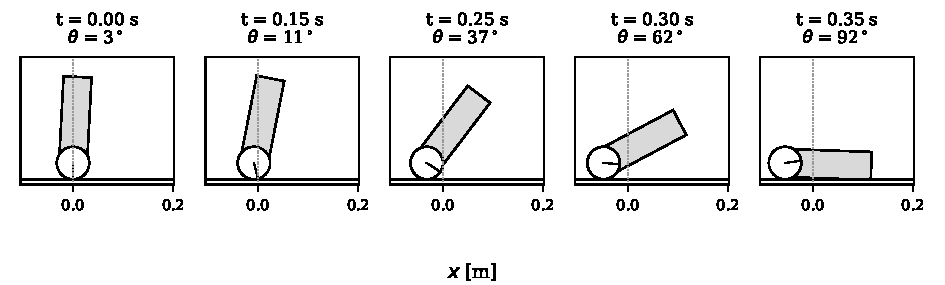
\includegraphics[width=\linewidth]{figures/free_fall_frames.pdf}
\caption{Free fall with the motor off (RK4, $\Delta t = \SI{5}{ms}$). The
dotted line marks the initial position of the axle.}
\label{fig:frames}
\end{figure}

\begin{figure}[h]
\centering
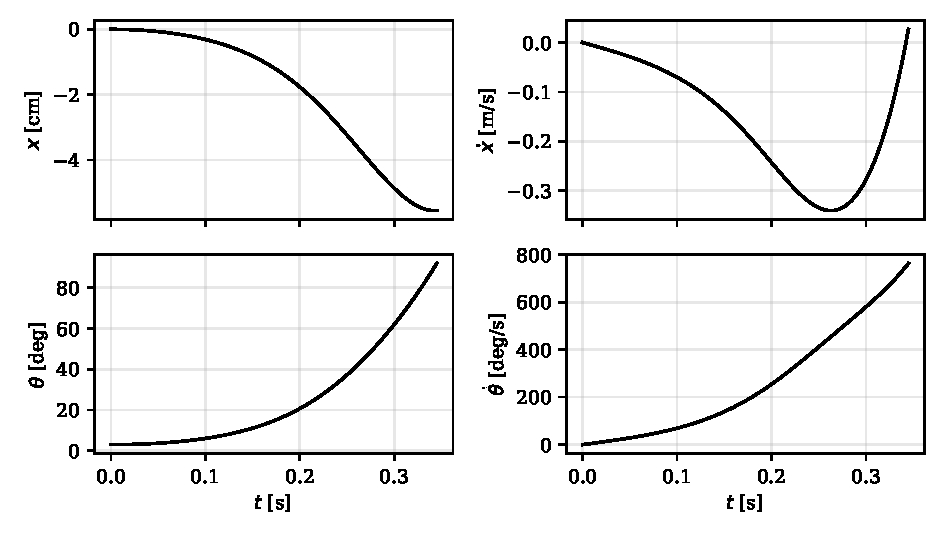
\includegraphics[width=\linewidth]{figures/free_fall_states.pdf}
\caption{State during the free fall (RK4, $\Delta t = \SI{5}{ms}$).}
\label{fig:states}
\end{figure}

The motion of the wheels follows from the equation of motion of $x$. With
$\tau = 0$, $Q_x = 0$ and $\partial L/\partial x = 0$, so \cref{eq:EL} reduces
to $\frac{\dd}{\dd t}\left(\partial L/\partial\dot x\right) = 0$: the
generalised momentum
\begin{equation}
  p_x = \frac{\partial L}{\partial\dot x} = a\,\dot x + \mb l\cos\theta\,\dot\theta
\end{equation}
is conserved. Starting from rest, $p_x = 0$ at all times, hence
\begin{equation}
  \dot x = -\frac{\mb l\cos\theta}{a}\,\dot\theta .
\end{equation}
A forward rotation of the body ($\dot\theta > 0$) therefore drives the wheels
backwards, through the coupling term $b = \mb l\cos\theta$, and the effect
vanishes at $\theta = 90^\circ$, where $\cos\theta = 0$. Along the simulated
trajectory $|p_x|$ stays below \SI{1.7e-8}{kg.m/s}.

\paragraph{Energy.} \Cref{fig:energy} shows the relative drift of the total
energy for the two integrators with the same step. The maximum drift is
\num{6.2e-3} with explicit Euler and \num{7.6e-8} with RK4. The Euler error
grows as the motion accelerates; RK4 conserves the energy to within the
accuracy required by the tests, and is the default integrator of the simulator.

\begin{figure}[h]
\centering
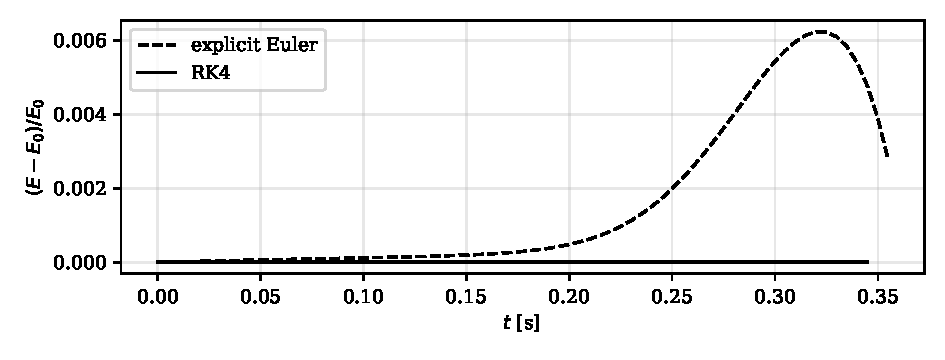
\includegraphics[width=\linewidth]{figures/free_fall_energy.pdf}
\caption{Relative drift of the total energy $E = T + V$ during the free fall,
explicit Euler and RK4, $\Delta t = \SI{5}{ms}$.}
\label{fig:energy}
\end{figure}
